%!TEX root = ../thesis.tex
%*******************************************************************************
%****************************** Second Chapter *********************************
%*******************************************************************************

\chapter{Contexte}
\label{chap:contexte}
\ifpdf
    \graphicspath{{Chapter3/Figs/Raster/}{Chapter3/Figs/PDF/}{Chapter3/Figs/}}
\else
    \graphicspath{{Chapter3/Figs/Vector/}{Chapter3/Figs/}}
\fi


Adversarial training

\section{Transfer learning}


Our problem is not about transfer learning after all.

\section{Representation learning}

Fairness


\section{+ Article de Younes}



\begin{figure}[htb]
  \centering
  \begin{subfigure}[t]{0.49\linewidth}
    
\includegraphics[width=\linewidth]{minion}
    \caption{Minions}
    \label{fig:minion}
  \end{subfigure}%
  \hfill
  \begin{subfigure}[t]{0.49\linewidth}
    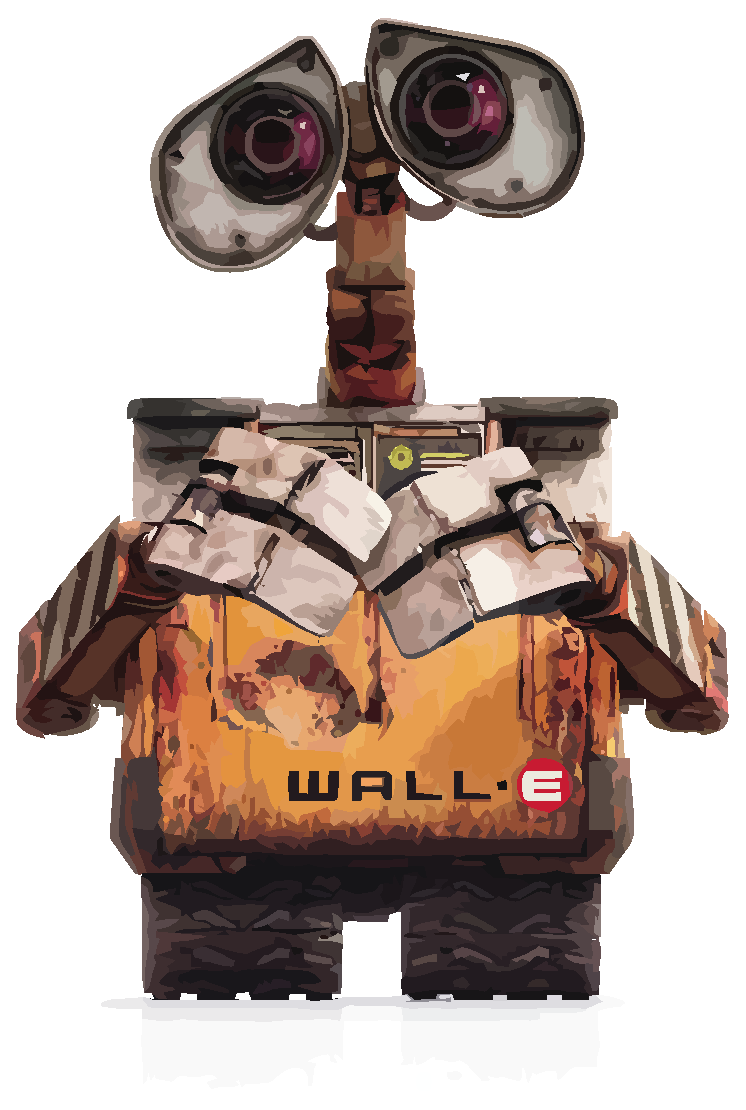
\includegraphics[width=\linewidth]{WallE}
    \caption{"Eve"}
    \label{fig:walle}
  \end{subfigure}
  \caption{Comparison Minions (left) and WallE (right)}
  \label{fig:comparision}
\end{figure}
